\chapter{Experiments and Results} \label{experiments}

\section{Background}

In this thesis, GNNs were used to predict the evolution of
complex dynamics on networks, specifically contagion dynamics
and majority rule dynamics. To this end, the publication
``Deep learning of contagion dynamics on complex networks''
by \citet{murphy} served as a basis both as an insipiration
and as a coding paradigm. In the approach used, dynamics of network
are learned through deep learning techniques, very few assumptions
are made about them. It is also demonstrated, that GNNs which
are usually used for structure learning, can also be used to model
complex dynamics on simple and complex networks, and that they
can provide predictions for previously unseen network structures allowing
for learned dynamics to be applied beyond the training data. 

\textbf{TODO: MAYBE MORE HERE}

\section{Fundamental Ideas of this approach}

In this approach, it is assumed that an unknown dynamical process
denoted as $M$ which takes places on a known network structure
$G = (V, E; \bm{\Phi}, \bm{\Omega})$ where $V$ is the node vector,
$E$ is the node set and $\bm{\Phi}_i$ and $\bm{\Omega}_{ij}$ are node
and edge attributes respectively, such as node attributes or edge weights. 
The dynamics acting on the network generate a time series $D$, defined as
pairs of consecutive spanshots $D = (\bm{X}, \bm{Y})$ with
$\bm{X} = (X_1, \cdots, X_T)$ the state of the nodes at time $t$ and
$\bm{Y} = {Y_1, \cdots, Y_T}$ the outcome of the dynamics with
$Y_t = M(X_t, G)$ with $X_t \in S^{|V|}$, $t, Y_t \in R^{|V|}$ where
$S$ is the set of possible node states and $R$ is the set possible node
outcomes. The elements $x_i(t) = (X_t)_i \text{ and } y_i(t) = (Y_t)_i$
correspond to the state of node $v_i$ at time $t$ and its outcome after
transitioning respectively, thus $S=R$ and it is possible to write
$y_i(t) = x_i(t + \Delta t)$ where $\Delta t$ is the length of the
time steps. If $S$ is a discrete set then $y_i(t)$ is a transition
probability vector and its value is sampled from a set of possible
values. In fact, $y_i(t)_m$ is the probability that node $v_i$ transitions
to state $m \in S$ if it was previously in $x_i(t)$ --- i.e. when studying
an SIS dynamics model that could be $R = [0,1]^{|S|}$. In stochastic dynamics'
modelling, the transition probabilities are not directly accessible, so
the observed outcome state is used to produce a definition for the observed
outcome $\tilde{y}_i(t)$:
\begin{equation}
  \tilde{y}_i(t)_m = \delta (x_i(t+\Delta t), m), \forall m \in S
\end{equation}

where $\delta$ is the Kronecker delta function. If the stochastic dynamics
$M$ used in this case is assumed to act on $X_t$ locally and identically
at all times, it is possible to compute the value of $y_i$ with a time
independent function identical for all nodes
\begin{equation}
  \label{eq:y_indepe}
  y_i = f(x_i, \Phi_i, x_{N_i}, \Phi_{N_i}, \Omega_{iN_i})
\end{equation}

where $N_i$ is the set of neighbors of node $v_i$. The result of this
process is a notion of locality of the underlying dynamics which also
is time-invariant and node-invariant (and edge-invariant) as required
and discussed in previous sections.

\section{Description of goals}
The goal of this approach is to build a model $\hat{M}$ with learnable
parameters $\bm{\Theta}$ which after being trained over a set of the
observed dataset D mimics $M$ given $G$ so that:
\begin{equation}
  \label{eq:M_mimicks}
  \hat{M}(X'_t, G'; \bm{\Theta}) \approx M(X'_t, G')
\end{equation}

The design of the GNN (discussed in more detail later) is based around
the notion of locality, imposed by a modified attention mechanism, which
allows for the arthitecture to be inductive; training on a wide range of
local structures makes it possible to use the model on any other network within
that local range. Therefore, the topology of the network is strongly associated
with the quality of the trained models. The node outcomes computed by the GNN
can be written in a similar manner as \eref{eq:y_indepe}:
\begin{equation}
  \label{eq:outcomes_y}
  \hat{y}_i = \hat{f}(x_i, \Phi_i, x_{N_i}, \Phi_{N_i}, \Omega_{iN_i}; \bm{\Theta})
\end{equation}

\textbf{Loss Function}: The loss function incorporates an arithmetic mean,
assuming all inputs are equally important and uniformly distributed. This is
critical as in practice that does not hold with finite number of inputs $D$ which
is not typically uniform and some parametrization is needed. The loss function
used in this model is:
\begin{equation}
  \label{eq:loss_func}
  L(\bm{\Theta}) = \sum_{t \in T'} \sum_{v_i \in V'(t)} \frac{w_i(t)}{Z'}L(y_i(t), \hat{y}_i(t))
\end{equation}

where $w_i(t)$ is the weight assigned to node $v_i$ at time $t$,
$Z'=\sum_{t \in T'} \sum_{v_i \in V'(t)}w_i(t)$ a normalization factor
and $L(y_i(t), \hat{y}_i(t))$ the local losses of each node.

\section{Architecture of the GNN}

\subsection{Structure}
\begin{figure}[H]
  \centering
  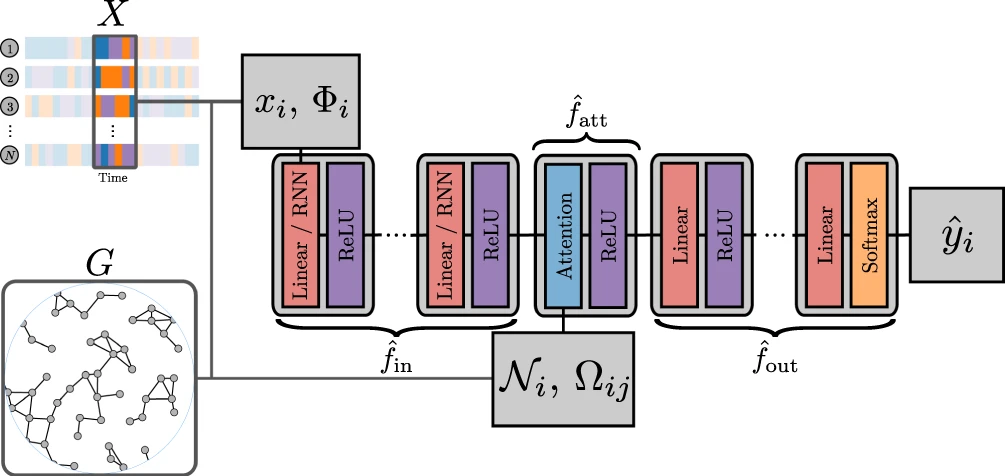
\includegraphics[width=\textwidth]{Figures/chap_exp/GATArch.png}
  \caption[The GAT GNN Architecture]{Schematic showing the layers in the GAT GNN used. Red blocks indicate trainable affine transformations (automorphisms). Purple blocks indicate activation functions. The attention module is in blue and the orange block in the end is the last activation which translates the transformations to the expected format. Image source \cite{murphy}.}
  \label{fig:GATGNN}
\end{figure}

The architecture of the network used can be seen in \fref{fig:GATGNN}.
The state $x_i$ of each node is transformed through a shared MLP
$\hat{f}_{in} : S \rightarrow \mathbb{R}^d$ where $d$ is the resulting
number of node features:
\begin{equation}
  \label{eq:input_layer}
  \xi_i = \hat{f}_{in}(x_i)
\end{equation}
When available, the node attributes $\Phi_i$ are concatenated to $x_i$
so $\hat{f}_{in}: S \times \mathbb{R}^Q \rightarrow \mathbb{R}^d$ and the
$\xi_i$ is now a feature vector with representing the state and attributes of node $v_i$.
The features of the first neighbors are then aggregated using an attention mechanism
discussed in the next section:
\begin{equation}
  \label{eq:first_att}
  v_i = \hat{f}_{att} (\xi_i, \xi_{N_i})
\end{equation}

If available, edge attributes $\Omega_{ij}$ are also included in the attention
mechanism. In a similar manner as before, these attributes are first transformed
into edge features through a $\psi_{ij} = \hat{f}_{edge} (\Omega_{ij})$ where
$\hat{f}_{edge}: \mathbb{R}^P \rightarrow \mathbb{R}^{d_edge}$ is also an MLP.
Finally the outcome $\hat{y}_i$ of each node is computed with another MLP $\hat{f}_{out}: \mathbb{R}^d \rightarrow R$:
\begin{equation}
  \label{eq:final_out}
  \hat{y}_i = \hat{f}_{out}(v_i)
\end{equation}

\subsection{Attention Mechanism}
The attention mechanism used is a modified version of the one described by
\citet{velickovic2017graph}. It consists of three trainable functions
$A, B \text{ and} C$ that combine the feature vectors $\xi_i, xi_j \text{ and } \psi_{ij}$ of
pair of connected nodes $v_i$ and $v_j$. The attention coefficient is:
\begin{equation}
  \label{eq:att_coeff}
  \alpha_{ij} = \sigma \big[ A(\xi_i) + B(\xi_j) + C(\psi_{ij}) \big]
\end{equation}
where $\sigma$ is the logistic function which allows for an output range
in $(0, 1)$, 1 meaning maximal influence of $v_j$ on $v_i$ and 0 non-existent influence.
All of the transformations $A, B, \text{ and } C$ are affine and have trainable weights
and biases. 

The aggregation formula is:
\begin{equation}
  \label{eq:att_aggr}
  v_i = \hat{f}_{att}(\xi_i, \xi_{N_i}) = \xi_i + \sum_{v_j \in N_i} \alpha_{ij} \xi_j
\end{equation}
and this $v_i$ contais information about itself and its neighbors through a
multi-head attention mechanism. In contrast with the proposed aggregation mechanism
from the GAT paper, the one used in \eref{eq:att_aggr} uses a general weighted sum
which allows for the architecture to express dynamic process more accurately. The one
used by the GAT paper and other architectures is better when creating models for structure
learning. 

\subsection{Loss Function}
The cross entropy loss function was used in all experiments:
\begin{equation}
  \label{eq:cross_loss}
  L(y_i, \hat{y}_i) = - \sum_m y_{i,m} log \hat{y}_{i,m}
\end{equation}
with $y_i,m$ the $m^{th}$ element of the outcome vector for node $v_i$ a transition
probability vector as discussed before. 
\section{Experiments TODO}
\subsection{SIS}
\subsection{Modular}
\subsection{Majority rule}